\documentclass[11pt]{article}
\usepackage{amsmath}
\usepackage{amssymb}
\usepackage{graphicx}
\usepackage{tabularx}
\usepackage{fancyhdr}
\usepackage{lastpage}

% Page layout
\usepackage[top=1in, bottom=1in, left=1in, right=1in]{geometry}

% Header and footer
\pagestyle{fancy}
\fancyhf{}
\rfoot{Page \thepage}
\renewcommand{\headrulewidth}{0pt}

% Modified Question command with left-aligned number
\newcommand{\questiona}[2]{
    \noindent\textbf{Q#2.} #1 \hfill \textbf{[1 Mark]}
}

\newcommand{\questionb}[2]{
    \noindent\textbf{Q#2.} #1 \hfill \textbf{[2 Marks]}
}

\begin{document}

% Title section with horizontal line
\begin{center}
    \Large\textbf{GATE 2018 - Chemistry (CY)} \\
    \large\textbf{General Aptitude and Technical Questions} \\
    \rule{\textwidth}{0.5pt} % Horizontal line below heading
\end{center}

\vspace{0.5cm}

% General Aptitude Section
\section*{General Aptitude}

\questiona{"When she fell down the \_\_\_\_\_, she received many \_\_\_\_\_ but little help." The words that best fill the blanks in the above sentence are}{1}
\begin{enumerate}
    \item[(A)] stairs, stares  
    \item[(B)] stairs, stairs  
    \item[(C)] stares, stairs  
    \item[(D)] stares, stares  
\end{enumerate}
\vspace{0.5cm}

\questiona{"In spite of being warned repeatedly, he failed to correct his \_\_\_\_\_ behaviour." The word that best fills the blank in the above sentence is}{2}
\begin{enumerate}
    \item[(A)] rational  
    \item[(B)] reasonable  
    \item[(C)] errant  
    \item[(D)] good  
\end{enumerate}
\vspace{0.5cm}

\questiona{For \(0 \leq x \leq 2\pi\), \(\sin x\) and \(\cos x\) are both decreasing functions in the interval \_\_\_\_\_.}{3}
\begin{enumerate}
    \item[(A)] \(\left(0, \frac{\pi}{2}\right)\)  
    \item[(B)] \(\left(\frac{\pi}{2}, \pi\right)\)  
    \item[(C)] \(\left(\pi, \frac{3\pi}{2}\right)\)  
    \item[(D)] \(\left(\frac{3\pi}{2}, 2\pi\right)\)  
\end{enumerate}
\vspace{0.5cm}

\questiona{The area of an equilateral triangle is \(\sqrt{3}\). What is the perimeter of the triangle?}{4}
\begin{enumerate}
    \item[(A)] 2  
    \item[(B)] 4  
    \item[(C)] 6  
    \item[(D)] 8  
\end{enumerate}
\vspace{0.5cm}

\questiona{Arrange the following three-dimensional objects in the descending order of their volumes:
\begin{enumerate}
    \item A cuboid with dimensions 10 cm, 8 cm and 6 cm
    \item A cube of side 8 cm
    \item A cylinder with base radius 7 cm and height 7 cm
    \item A sphere of radius 7 cm
\end{enumerate}}{5}
\begin{enumerate}
    \item[(A)] (i), (ii), (iii), (iv)
    \item[(B)] (ii), (i), (iv), (iii)
    \item[(C)] (iii), (ii), (i), (iv)
    \item[(D)] (iv), (iii), (ii), (i)
\end{enumerate}
\vspace{0.5cm}

\questionb{An automobile travels from city A to city B and returns to city A by the same route. The speed of the vehicle during the onward and return journeys were constant at 60 km/h and 90 km/h, respectively. What is the average speed in km/h for the entire journey?}{6}
\begin{enumerate}
    \item[(A)] 72  
    \item[(B)] 73  
    \item[(C)] 74  
    \item[(D)] 75  
\end{enumerate}
\vspace{0.5cm}

\questionb{A set of 4 parallel lines intersect with another set of 5 parallel lines. How many parallelograms are formed?}{7}
\begin{enumerate}
    \item[(A)] 20  
    \item[(B)] 48  
    \item[(C)] 60  
    \item[(D)] 72  
\end{enumerate}
\vspace{0.5cm}

\questionb{To pass a test, a candidate needs to answer at least 2 out of 3 questions correctly. A total of 6,30,000 candidates appeared for the test. Question A was correctly answered by 3,30,000 candidates. Question B was answered correctly by 2,50,000 candidates. Question C was answered correctly by 2,60,000 candidates. Both questions A and B were answered correctly by 1,00,000 candidates. Both questions B and C were answered correctly by 90,000 candidates. Both questions A and C were answered correctly by 80,000 candidates. If the number of students answering all questions correctly is the same as the number answering none, how many candidates failed to clear the test?}{8}
\begin{enumerate}
    \item[(A)] 30,000  
    \item[(B)] 2,70,000  
    \item[(C)] 3,90,000  
    \item[(D)] 4,20,000  
\end{enumerate}
\vspace{0.5cm}

\questionb{If \(x^2 + x - 1 = 0\) what is the value of \(x^4 + \frac{1}{x^4}\)?}{9}
\begin{enumerate}
    \item[(A)] 1  
    \item[(B)] 5  
    \item[(C)] 7  
    \item[(D)] 9  
\end{enumerate}
\vspace{0.5cm}

\questionb{In a detailed study of annual crow births in India, it was found that there was relatively no growth during the period 2002 to 2004 and a sudden spike from 2004 to 2005. In another unrelated study, it was found that the revenue from cracker sales in India which remained fairly flat from 2002 to 2004, saw a sudden spike in 2005 before declining again in 2006. The solid line in the graph below refers to annual sale of crackers and the dashed line refers to the annual crow births in India. Choose the most appropriate inference from the above data.}{10}
\begin{center}
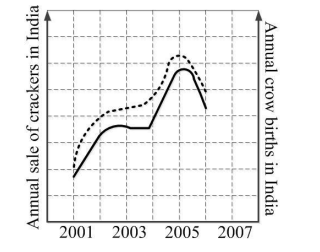
\includegraphics[width=0.5\textwidth]{figures/10.png}
\end{center}
\begin{enumerate}
    \item[(A)] There is a strong correlation between crow birth and cracker sales.
    \item[(B)] Cracker usage increases crow birth rate.
    \item[(C)] If cracker sale declines, crow birth will decline.
    \item[(D)] Increased birth rate of crows will cause an increase in the sale of crackers.
\end{enumerate}
\vspace{0.5cm}

% Technical Section
\section*{Technical Section}

\questiona{The major product formed in the following reaction is}{1}
\begin{center}
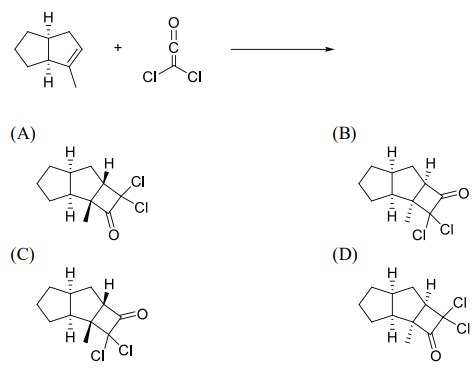
\includegraphics[width=0.8\textwidth]{figures/1}
\end{center}

\vspace{0.5cm}

\questiona{The major product formed in the following reaction is}{2}
\begin{center}
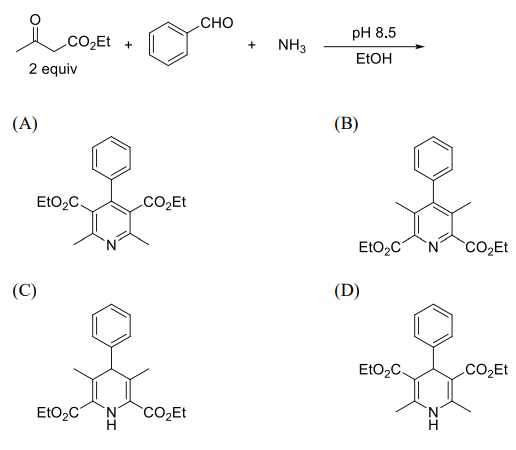
\includegraphics[width=0.8\textwidth]{figures/2}
\end{center}

\vspace{0.5cm}

\questiona{The major product of the following intramolecular cycloaddition reaction is}{3}
\begin{center}
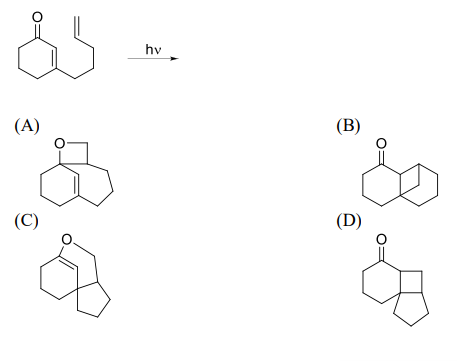
\includegraphics[width=0.8\textwidth]{figures/3}
\end{center}

\vspace{0.5cm}

\questiona{The major product of the following reaction is}{4}
\begin{center}
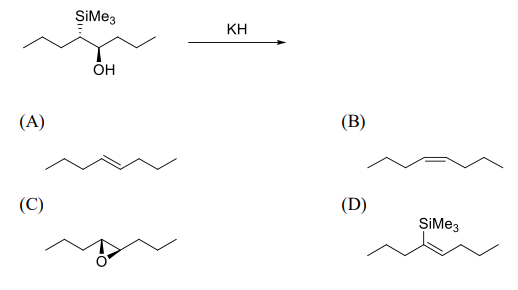
\includegraphics[width=0.8\textwidth]{figures/4}
\end{center}

\vspace{0.5cm}

\questiona{The major product formed in the following reaction sequence is}{5}
\begin{center}
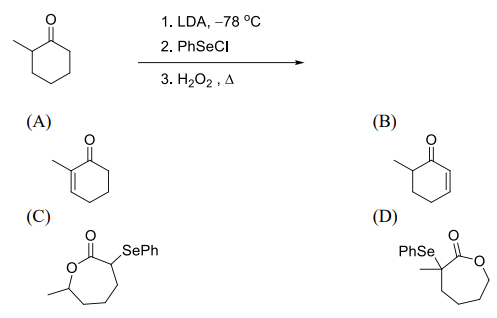
\includegraphics[width=0.8\textwidth]{figures/5}
\end{center}

\vspace{0.5cm}

\questiona{The major product formed in the following reaction sequence is}{6}
\begin{center}
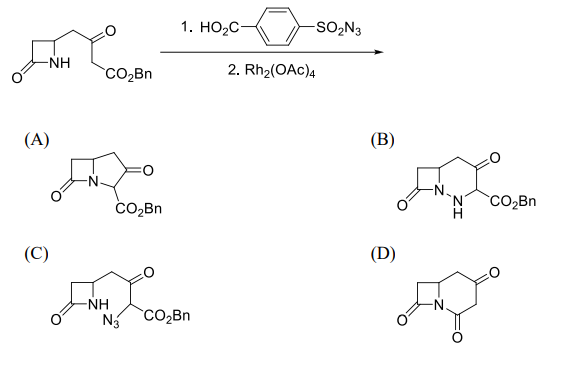
\includegraphics[width=0.8\textwidth]{figures/6.png}
\end{center}

\vspace{0.5cm}

\questiona{The spherical harmonic function, \( Y_{lm}(\theta,\phi) \), with appropriate values of \( l \) and \( m \), is an eigenfunction of \( \hat{L}_x^2 + \hat{L}_y^2 \) operator. The corresponding eigenvalue is}{7}
\begin{enumerate}
    \item[(A)] \( l(l+1)\hbar^2 \)
    \item[(B)] \( \left( l(l+1)+m^2 \right) \hbar^2 \)
    \item[(C)] \( \left( l(l+1)-m^2 \right) \hbar^2 \)
    \item[(D)] \( m^2\hbar^2 \)
\end{enumerate}
\vspace{0.5cm}

\questiona{Consider the operators, \(\hat{a}_+ = \frac{1}{\sqrt{2}} (\hat{x} + i\hat{p}_x)\) and \(\hat{a}_- = \frac{1}{\sqrt{2}} (\hat{x} - i\hat{p}_x)\), where \(\hat{x}\) and \(\hat{p}_x\) are the position and linear momentum operators, respectively. The commutator, \([\hat{a}_+, \hat{a}_-]\), is equal to}{8}
\begin{enumerate}
    \item[(A)] \(i\hbar\)
    \item[(B)] \(-i\hbar\)
    \item[(C)] \(\hbar\)
    \item[(D)] \(-\hbar\)
\end{enumerate}
\vspace{0.5cm}

\questiona{The temperature derivative of electrochemical cell potential \(E\) at constant pressure, \(\left( \frac{\partial E}{\partial T} \right)_p\), is given by}{9}
\begin{enumerate}
    \item[(A)] \(-\frac{\Delta S}{nF}\)
    \item[(B)] \(\frac{\Delta S}{nF}\)
    \item[(C)] \(\frac{\Delta S}{nFT}\)
    \item[(D)] \(-\frac{\Delta S}{nFT}\)
\end{enumerate}
\vspace{0.5cm}

\questiona{For an ionic micelle-forming surfactant near its critical micelle concentration (CMC), the dependence of molar conductivity and surface tension on surfactant concentration is best represented by}{10}
\begin{center}
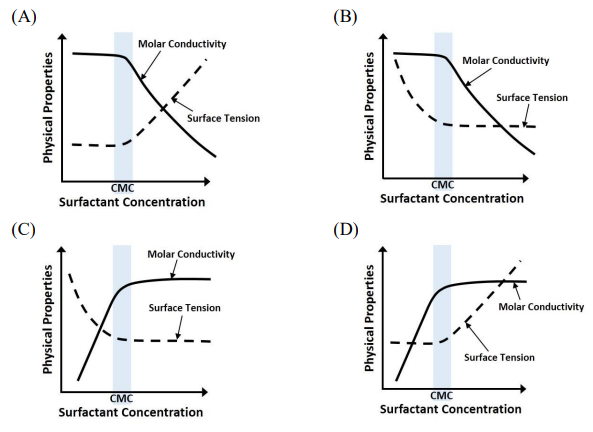
\includegraphics[width=0.8\textwidth]{figures/10a.png}
\end{center}
\vspace{0.5cm}

\questiona{According to Eyring transition state theory for a bimolecular reaction, the activated complex has}{11}
\begin{enumerate}
    \item[(A)] no vibrational degrees of freedom.
    \item[(B)] vibrational degrees of freedom but they never participate in product formation.
    \item[(C)] one high frequency vibration that leads to product formation.
    \item[(D)] one low frequency vibration that leads to product formation.
\end{enumerate}
\vspace{0.5cm}

\questiona{Based on Wade's rule, the structure-type of $[B_5H_5]^{-1}$ is}{12}
\begin{enumerate}
    \item[(A)] closo
    \item[(B)] nido
    \item[(C)] arachno
    \item[(D)] hypho
\end{enumerate}
\vspace{0.5cm}

\questiona{The coordination geometries around the copper ion of plastocyanin (a blue-copper protein) in oxidized and reduced form, respectively, are}{13}
\begin{enumerate}
    \item[(A)] tetrahedral and square-planar
    \item[(B)] square-planar and tetrahedral
    \item[(C)] distorted tetrahedral for both
    \item[(D)] ideal tetrahedral for both
\end{enumerate}
\vspace{0.5cm}

\questiona{The water exchange rates for the complex ions follow the order}{14}
\begin{enumerate}
    \item[(A)] $[V(H_2O)_6]^{2+} > [Co(H_2O)_6]^{2+} > [Cr(H_2O)_6]^{3+}$
    \item[(B)] $[Cr(H_2O)_6]^{3+} > [Co(H_2O)_6]^{2+} > [V(H_2O)_6]{2+}$
    \item[(C)] $[Co(H_2O)_6]^{2+} > [Cr(H_2O)_6]^{3+} > [V(H_2O)_6]{2+}$
    \item[(D)] $[Co(H_2O)_6]^{2+} > [V(H_2O)_6]{2+} > [Cr(H_2O)_6]^{3+}$
\end{enumerate}
\vspace{0.5cm}

\questiona{The lowest energy \( d \rightarrow d \) transition of the complexes follow the order}{15}
\begin{enumerate}
    \item[(A)] $[Cr(H_2O)_6]^{3+} < [Cr(NH_3)_6]{3+} < [Cr(CN)_6]^{3+}$
    \item[(B)] $[Cr(CN)_6]^{3+}< [Cr(NH_3)_6]{3+} < [Cr(H_2O)_6]^{3+}$
    \item[(C)] $[Cr(CN)_6]^{3+}< [Cr(H_2O)_6]^{3+} < [Cr(NH_3)_6]{3+}$
    \item[(D)] $[Cr(NH_3)_6]{3+} < [Cr(CN)_6]^{3+} < [Cr(H_2O)_6]^{3+}$
\end{enumerate}
\vspace{0.5cm}

\questiona{The symmetry label of valence p orbitals of a metal ion in an octahedral ligand field is}{16}
\begin{enumerate}
    \item[(A)] t1g
    \item[(B)] t1u
    \item[(C)] eg + a1g
    \item[(D)] t2g
\end{enumerate}
\vspace{0.5cm}

\questiona{The bond angle (Ti-C-C) in the crystal structure of 
\begin{center}
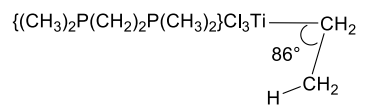
\includegraphics[width=0.5\textwidth]{figures/17.png}
\end{center}
is severely distorted due to}{17}
\begin{enumerate}
    \item[(A)] hydrogen-bonding interaction
    \item[(B)] agostic interaction
    \item[(C)] steric bulk of the phosphine ligand
    \item[(D)] higher formal charge on metal
\end{enumerate}
\vspace{0.5cm}

\questiona{The molar heat capacity of a substance is represented in the temperature range 298 K to 400 K by the empirical relation \( C_{p,m} = 14 + bT \) J $K^{-1} mol^{-1}$, where b is a constant. The molar enthalpy change when the substance is heated from 300 K to 350 K is 2 kJ $mol^{-1}$. The value of b is \_\_\_\_\_ J $K^{-2} mol^{-1}$. (Up to two decimal places)}{18}
\vspace{0.5cm}

\questiona{For low partial pressure of ozone ($O_3$), the adsorption of ozone on graphite surface is fully dissociative in nature, and follows Langmuir isotherm. Under these conditions, if the dependence of the surface coverage of graphite \(\theta\) on partial pressure of ozone $P_{O3}$ is given by $\theta \propto (P_{O3})^x)$, the value of x is \_\_\_\_\_. (Up to two decimal places)}{19}
\vspace{0.5cm}

\questiona{For the radioactive isotope \(^{131}\)I, the time required for 50\% disintegration is 8 days. The time required for the 99.9\% disintegration of 5.5 g of \(^{131}\)I is \_\_\_\_\_ days. (Up to one decimal place)}{20}
\vspace{0.5cm}

\questiona{Two moles of an ideal gas X and two moles of an ideal gas Y, initially at the same temperature and pressure, are mixed under isothermal-isobaric condition. The entropy change on mixing is \_\_\_\_\_ J $K^{-1}$. (Up to one decimal place. Use \(R = 8.31\) J $K^{-1}$ $mol^-1$)}{21}
\vspace{0.5cm}

\questiona{The energy of a hydrogen molecule in its ground state equilibrium configuration is -31.7 eV. Its dissociation energy is \_\_\_\_\_ eV. (Up to one decimal place)}{22}
\vspace{0.5cm}

\questiona{The total number of valence electrons in W(\(\eta^3\)-Cp)(\(\eta^5\)-Cp)$(CO)_2$ is \_\_\_\_\_. (Atomic number of W = 74)}{23}
\vspace{0.5cm}

\questiona{In the \(^1\)H NMR spectrum of an organic compound recorded on a 300 MHz instrument, a proton resonates as a quartet at \(\delta\) 4.20 ppm. The individual signals of the quartet appear at \(\delta\) 4.17, 4.19, 4.21 and 4.23 ppm. The coupling constant \(J\) in Hz is \_\_\_\_\_.}{24}
\vspace{0.5cm}

\questiona{In the electron ionization (EI) mass spectra, methyl hexanoate, methyl heptanoate and methyl octanoate give the same base peak. The m/z value of the base peak is \_\_\_\_\_.}{25}
\vspace{0.5cm}

\questionb{In the following reaction,}{26}
\begin{figure}[h]
\centering
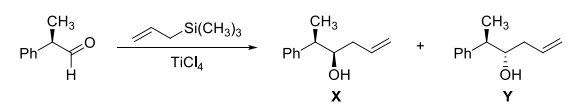
\includegraphics[width=0.5\textwidth]{figures/26}
\end{figure}
\begin{enumerate}
    \item[(A)] X is the major product and Y is the minor product
    \item[(B)] X is the only product
    \item[(C)] Y is the only product
    \item[(D)] X is the minor product and Y is the major product
\end{enumerate}
\vspace{0.5cm}

\questionb{The enantiomeric pair, among the following, is}{27}
\begin{center}
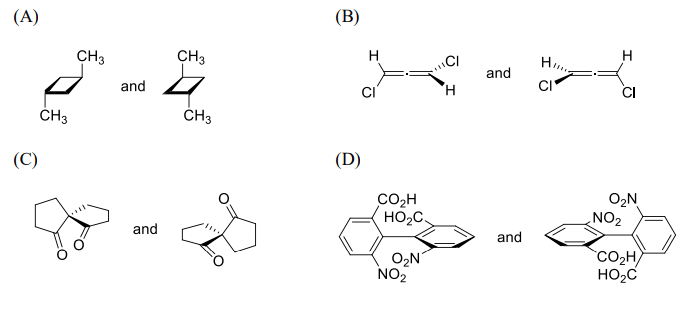
\includegraphics[width=0.8\textwidth]{figures/27.png}
\end{center}
\vspace{0.5cm}

\questionb{The major product formed in the following reaction sequence is}{28}
\begin{center}
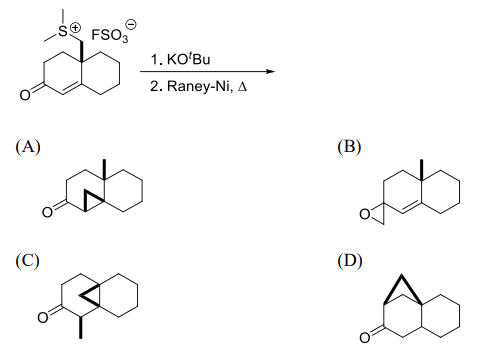
\includegraphics[width=0.8\textwidth]{figures/28.png}
\end{center}

\vspace{0.5cm}

\questionb{The major product in the following reaction sequence is}{29}
\begin{center}
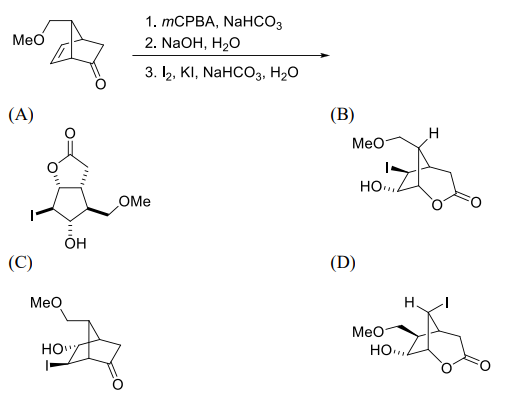
\includegraphics[width=0.8\textwidth]{figures/29.png}
\end{center}

\vspace{0.5cm}

\questionb{The major product formed in the following reaction sequence is}{30}
\begin{center}
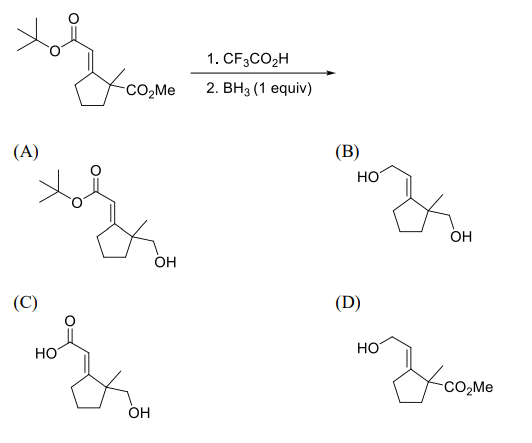
\includegraphics[width=0.8\textwidth]{figures/30.png}
\end{center}

\vspace{0.5cm}

\questionb{The major product of the following reaction sequence is}{31}
\begin{center}
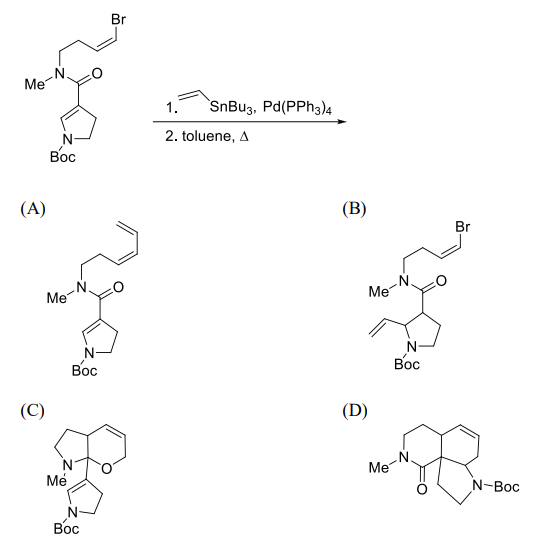
\includegraphics[width=0.8\textwidth]{figures/31.png}
\end{center}

\vspace{0.5cm}

\questionb{The major product formed in the following retro-aldol reaction is}{32}
\begin{center}
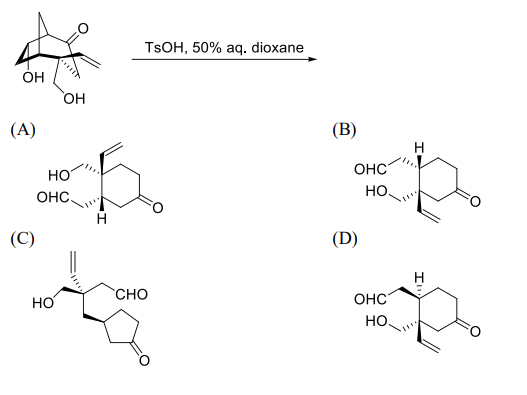
\includegraphics[width=0.8\textwidth]{figures/32.png}
\end{center}

\vspace{0.5cm}

\questionb{The elimination product of the following reaction is}{33}
\begin{center}
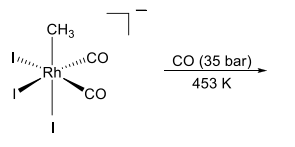
\includegraphics[width=0.8\textwidth]{figures/33.png}
\end{center}
\begin{enumerate}
    \item[(A)] I$_2$
    \item[(B)] CH$_3$I
    \item[(C)] CH$_3$COI
    \item[(D)] I$_3^-$
\end{enumerate}
\vspace{0.5cm}

\questionb{A one-dimensional anharmonic oscillator is treated by perturbation theory. The harmonic oscillator is used as the unperturbed system and the perturbation is $\frac{1}{6}\gamma x^3$ ($\gamma$ is a constant). Using only the first order correction, the total ground state energy of the anharmonic oscillator is}{34}
\begin{enumerate}
    \item[(A)] $\frac{1}{2}\hbar\left(\frac{k}{\mu}\right)^{1/2}$
    \item[(B)] $\left(\frac{1}{2} + \frac{\gamma}{6}\right)\hbar\left(\frac{k}{\mu}\right)^{1/2}$
    \item[(C)] $\left(\frac{1}{2} + \frac{\gamma}{3}\right)\hbar\left(\frac{k}{\mu}\right)^{1/2}$
    \item[(D)] $\left(\frac{1}{2} + \frac{\gamma}{12}\right)\hbar\left(\frac{k}{\mu}\right)^{1/2}$
\end{enumerate}
\vspace{0.5cm}

\questionb{The O$_2$ coordinated to metal ion centres in oxy-myoglobin and oxy-hemocyanin exists, respectively, as}{35}
\begin{enumerate}
    \item[(A)] superoxide and peroxide
    \item[(B)] superoxide and superoxide
    \item[(C)] peroxide and peroxide
    \item[(D)] superoxide and oxygen
\end{enumerate}
\vspace{0.5cm}

\questionb{Spectroscopic ground state term symbols of cobalt ions in [Co(H$_2$O)$_6$]$^{2+}$ and [CoCl$_4$]$^{2-}$, respectively, are}{36}
\begin{enumerate}
    \item[(A)] $^2$T$_{1g}$ and $^4$A$_2$
    \item[(B)] $^4$T$_{1g}$ and $^4$A$_2$
    \item[(C)] $^4$T$_{2g}$ and $^4$T$_1$
    \item[(D)] $^2$T$_1$ and $^4$A$_1$
\end{enumerate}
\vspace{0.5cm}

\questionb{Generally, the coordination number and the nature of the electronic absorption band ($f \rightarrow f$ transition) of lanthanide(III) ion in their complexes are, respectively,}{37}
\begin{enumerate}
    \item[(A)] greater than 6 and sharp
    \item[(B)] 6 and broad
    \item[(C)] less than 6 and sharp
    \item[(D)] greater than 6 and broad
\end{enumerate}
\vspace{0.5cm}

\questionb{Second-order rate constant for the reaction between [Co(NH$_3$)$_5$X]$^{n+}$ (n = 3 for X = NH$_3$ and H$_2$O; n = 2 for X = Cl$^-$) and [Cr(H$_2$O)$_6$]$^{2+}$ at room temperature varies with the X as}{38}
\begin{enumerate}
    \item[(A)] NH$_3$ > H$_2$O > Cl$^-$
    \item[(B)] Cl$^-$ > H$_2$O > NH$_3$
    \item[(C)] NH$_3$ > Cl$^-$ > H$_2$O
    \item[(D)] H$_2$O > NH$_3$ > Cl$^-$
\end{enumerate}
\vspace{0.5cm}

\questionb{For the following reaction sequence,}{39}
\begin{center}
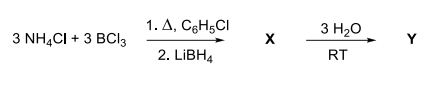
\includegraphics[width=0.8\textwidth]{figures/39.png}
\end{center}
X and Y, respectively, are
\begin{enumerate}
    \item[(A)] \{HB(NH)\}$_3$ and \{H(OH)B(NH$_2$)\}$_3$
    \item[(B)] \{HB(NH)\}$_3$ and \{HB(NH$_2$OH)\}$_3$
    \item[(C)] [NH$_4$][H$_2$(BH$_2$)$_3$] and \{H(OH)(NH$_2$OH)\}$_3$
    \item[(D)] [NH$_4$][H$_2$(BH$_2$)$_3$] and \{HB(NH$_2$OH)\}$_3$
\end{enumerate}
\vspace{0.5cm}

\questionb{For an inverse spinel, AB$_2$O$_4$, the A and B, respectively, can be}{40}
\begin{enumerate}
    \item[(A)] Ni(II) and Ga(III)
    \item[(B)] Zn(II) and Fe(III)
    \item[(C)] Fe(II) and Cr(III)
    \item[(D)] Mn(II) and Mn(III)
\end{enumerate}
\vspace{0.5cm}

\questionb{The reaction of PCl$_3$ with PhLi in 1:3 molar ratio yields X as one of the products, which on further treatment with CH$_3$I gives Y. The reaction of Y with n-BuLi gives product Z. The products X, Y and Z, respectively, are}{41}
\begin{enumerate}
    \item[(A)] [PPh$_4$]Cl, [Ph$_2$P=CH$_2$] and Ph$_2$P(n-Bu)
    \item[(B)] PPh$_3$, [Ph$_3$P][I(CH$_3$)] and Ph$_2$P(n-Bu)$_3$
    \item[(C)] PPh$_3$, [Ph$_3$P(CH$_3$)]I and Ph$_3$P=CH$_2$
    \item[(D)] [PPh$_4$]Cl, [Ph$_3$P=CH$_2$] and [Ph$_3$P(n-Bu)]Li
\end{enumerate}
\vspace{0.5cm}

\questionb{The reaction of equimolar quantities of Fe(CO)$_5$ and OH$^-$ gives a complex species X which on further reaction with MnO$_2$ gives species Y. X and Y, respectively, are}{42}
\begin{enumerate}
    \item[(A)] [Fe(CO)$_5$(OH)]$^-$ and Fe$_2$(CO)$_9$
    \item[(B)] [Fe(CO)$_4$]$^{2-}$ and Mn$_2$(CO)$_{10}$
    \item[(C)] [HFe(CO)$_4$]$^-$ and Fe$_2$O$_3$
    \item[(D)] [HFe(CO)$_4$]$^-$ and Fe$_3$(CO)$_{12}$
\end{enumerate}
\vspace{0.5cm}

\questionb{The rate constant of a first order reaction, X → Y, is $1.6 \times 10^{-3}$ s$^{-1}$ at 300 K. Given that the activation energy of the reaction is 28 kJ mol$^{-1}$ and assuming Arrhenius behavior for the temperature dependence, the total time required to obtain 90\% of Y at 350 K is \_\_\_\_\_ s. (Up to one decimal place. Use R = 8.31 J K$^{-1}$ mol$^{-1}$.)}{43}
\vspace{0.5cm}

\questionb{The molar conductivity of a 0.01 M weak acid (HX) at 298 K, measured in a conductivity cell with cell constant of 0.4 cm$^{-1}$, is 64.4 S cm$^2$ mol$^{-1}$. The limiting molar conductivities at infinite dilution of H$^+$ and X$^-$ at 298 K are 350 and 410 S cm$^2$ mol$^{-1}$, respectively. Ignoring activity coefficients, the pKa of HX at 298 K is \_\_\_\_\_. (Up to two decimal places)}{44}
\vspace{0.5cm}

\questionb{The Latimer diagram of oxygen is given below. The value of x is \_\_\_\_\_ V. (Up to two decimal places)}{45}
\begin{figure}[h]
\centering
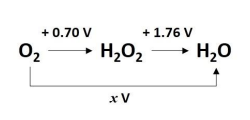
\includegraphics[width=0.5\textwidth]{figures/45}
\end{figure}
\vspace{0.5cm}

\questionb{At temperature T, the canonical partition function of a harmonic oscillator with fundamental frequency ($\mu$) is given by}{46}
\[ q_{vib}(T) = \frac{e^{-h\mu/2k_BT}}{1 - e^{-h\mu/k_BT}} \]
For $\frac{h\mu}{k_BT} = 3$, the probability of finding the harmonic oscillator in its ground vibrational state is \_\_\_\_\_. (Up to two decimal places)
\vspace{0.5cm}

\questionb{The enthalpy of vaporization of a liquid at its boiling point (T$_b$ = 200 K) is 15.3 kJ mol$^{-1}$. If the molar volumes of the liquid and the vapour at 200 K are 110 and 12000 cm$^3$ mol$^{-1}$ respectively, then the slope $\frac{dP}{dT}$ of the liquid-vapour boundary is \_\_\_\_\_ kPa K$^{-1}$. (Up to two decimal places. Note: 1 Pa = 1 J m$^{-3}$)}{47}
\vspace{0.5cm}

\questionb{In a molecule XY, let $\psi_x$ and $\psi_y$ denote normalized atomic orbitals of atoms X and Y, respectively. A normalized molecular orbital of XY is given by $\psi_+$ = 0.56($\psi_x$ + $\psi_y$). The value of the overlap integral of $\psi_x$ and $\psi_y$ is \_\_\_\_\_. (Up to two decimal places)}{48}
\vspace{0.5cm}

\questionb{The absorption maxima of two dyes X and Y are 520 and 460 nm, respectively. The absorbance data of these dyes measured in a 1 cm path length cell are given in the table below.}{49}
\begin{center}
\begin{tabular}{|c|c|c|}
\hline
Dye solution & Absorbance at 460 nm & Absorbance at 520 nm \\
\hline
X (9 mM) & 0.144 & 0.765 \\
Y (12 mM) & 0.912 & 0.168 \\
Mixture of X and Y & 0.700 & 0.680 \\
\hline
\end{tabular}
\end{center}
The concentration of Y in the mixture is \_\_\_\_\_ mM. (Up to two decimal places)
\vspace{0.5cm}

\questionb{The $\pi$ electrons in benzene can be modelled as particles in a ring that follow Pauli's exclusion principle. Given that the radius of benzene is 1.4 Å, the longest wavelength of light that is absorbed during an electronic transition in benzene is \_\_\_\_\_ nm. (Up to one decimal place. Use m$_e$ = 9.1 × 10$^{-31}$ kg, h = 6.6 × 10$^{-34}$ J s, c = 3.0 × 10$^8$ m s$^{-1}$)}{50}
\vspace{0.5cm}

\questionb{The spacing between the two adjacent lines of the microwave spectrum of H$^{35}$Cl is 6.35 × 10$^{11}$ Hz. Given that the bond length of D$^{35}$Cl is 5\% greater than that of H$^{35}$Cl, the corresponding spacing for D$^{35}$Cl is \_\_\_\_\_ × 10$^{11}$ Hz. (Up to two decimal places)}{51}
\vspace{0.5cm}

\questionb{For a diatomic vibrating rotor, in vibrational level v = 3 and rotational level J, the sum of the rotational and vibrational energies is 11493.6 cm$^{-1}$. Its equilibrium oscillation frequency is 2998.3 cm$^{-1}$, anharmonicity constant is 0.0124 and rotational constant under rigid rotor approximation is 9.716 cm$^{-1}$. The value of J is \_\_\_\_\_. (Up to nearest integer)}{52}
\vspace{0.5cm}

\questionb{Number of carbonyl groups present in the final product of the following reaction sequence is \_\_\_\_\_.}{53}
\begin{center}
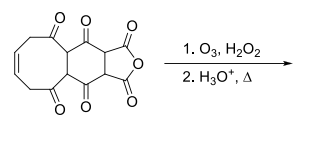
\includegraphics[width=0.5\textwidth]{figures/53.png}
\end{center}
\vspace{0.5cm}

\questionb{A tetrapeptide, made up of natural amino acids, has alanine as the N-terminal residue which is coupled to a chiral amino acid. Upon complete hydrolysis, the tetrapeptide gives glycine, alanine, phenylalanine and leucine. The number of possible sequences of the tetrapeptide is \_\_\_\_\_.}{54}
\vspace{0.5cm}

\questionb{The strongest band observed in the IR spectrum of the final product of the following reaction appears, approximately, at \_\_\_\_\_ × 100 cm$^{-1}$. (Up to one decimal place)}{55}
\begin{center}
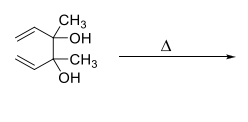
\includegraphics[width=0.5\textwidth]{figures/55.png}
\end{center}
\vspace{0.5cm}

\begin{center}
\textbf{END OF THE QUESTION PAPER}
\rule{\textwidth}{0.5pt} 
\end{center}

\end{document}
